\chapter{Stand van zaken}
\label{ch:stand-van-zaken}

% Tip: Begin elk hoofdstuk met een paragraaf inleiding die beschrijft hoe
% dit hoofdstuk past binnen het geheel van de bachelorproef. Geef in het
% bijzonder aan wat de link is met het vorige en volgende hoofdstuk.

% Pas na deze inleidende paragraaf komt de eerste sectiehoofding.

Dit hoofdstuk is een literatuurstudie over de huidige stand van zaken rond Kotlin. Hierin wordt bekeken wat Kotlin eigenlijk is, waarom Kotlin is uitgevonden. Daarna is Kotlin op verschillende platformen aan de beurt, meer specifieke is dit iOS, Android, web-applicatie en als back-end. Tenslotte het gebruik van Kotlin, hoeveel ontwikkelaars maken er reeds gebruik van Kotlin? Na het lezen van dit hoofdstuk bent u volledig op de hoogte van de laatste updates van Kotlin.

\section{Wat is Kotlin}
\label{sec:kotlin}
Kotlin is een open-source programmeertaal die object-georiënteerde en functionele programmatie features combineert. Kotlin is ook een statically typed programmeertaal. Dit betekent het type van de variabele is toegekend wanneer de code wordt gecompileerd. 
Javascript is een dynamically typed programmeertaal, waarbij je aan een variabele verschillende types kan toekennen. Zo kan een variabele bij Javascript in het begin een getal zijn, maar een beetje verder in de code kan dit veranderd worden naar een tekst.
\newline
\newline
Kotlin is ontworpen door JetBrains. JetBrains is een organisatie afkomstig van Sint-Petersburg, Rusland. De naam 'Kotlin' is afkomstig van het Kotlin eiland, 30 km ten westen van Sint-Petersburg. JetBrains is een software ontwikkeling bedrijf dat gesticht is in het jaar 2000. Hun hoofdkantoor is gevestigd in Praag, Tjsechië. Hun core-business is het ontwikkelen van tools die gebruikt kunnen worden door verschillende types van software ontwikkelaars. Zo hebben zij IDE's\footnote{Integrated Development Environment} ontwikkeld voor Java, Ruby, Python, PHP, SQL, Objective-C, C++, C\# en JavaScript.

\section{Kotlin en Android}
\label{sec:kotlinandroid}
In 2017 heeft Google bekend gemaakt dat het Kotlin volledig zou ondersteunen voor Android applicatieontwikkeling. Een Kotlin project maken in Android Studio is dan ook heel gemakkelijk. In Android Studio 3.0 heb je bij het aanmaken van een project de mogelijkheid om direct de ondersteuning voor Kotlin in te schakelen. Hierdoor zal je aangemaakte project onmiddelijk in Kotlin geschreven zijn.

Wil je bij een reeds bestaand project gebruik maken van Kotlin, dan zal je voor de klassen die je wenst om te zetten naar Kotlin, de actie 'Convert Java File to Kotlin File' moeten uitvoeren. Hierbij zal Android Studio detecteren dat er gebruik gemaakt wordt van Kotlin, waardoor hij zal vragen om de Kotlin plugin te installeren via Gradle.

\section{Automigration}
\label{sec:Automigration}
Door de intergratie van Kotlin in Android Studio werd er een conversietool ter beschikking gesteld. Met behulp van deze tool kan bestaande Java-code eenvoudig worden omgezet naar Kotlin. Dit zorgt ervoor dat veel tijd kan worden bespaard en het programmeren van dubbele code wordt zo vermeden. Maar deze conversietool bevat wel een klein risico. Het kan wel eens gebeuren dat code soms fout wordt geconverteerd. 

Het is ook reeds mogelijk om zowel Java en Kotlin te combineren. Zo kunnen de verschillende object classes in Java worden geschreven en kan je via Kotlin alle objecten aanmaken. Of dit nuttig en best practice is, is te beslissen door de developer.

\section{Kotlin web en back-end}
\label{sec:kotlincrossplatform}
Kotlin kan net zoals Java gebruikt worden om webapplicaties te bouwen. Dit in combinatie met bijvoorbeeld het Spring Framework, waarbij HttpServlets gebruikt worden om de webpagina's te tonen.

Wens je echter een full-stack webapplicatie te bouwen, dan heb je de mogelijkheid om ook een Kotlin server op te zetten. Zo kan je bijvoorbeeld aan de webapplicatie een RESTfull server hangen om verschillende API calls te doen.

Kotlin-applicaties kunnen worden geïmplementeerd op elke host die Java-webapplicaties ondersteunt, inclusief Amazon Web Services, Google Cloud Platform en veel meer.

\section{Kotlin Native}
\label{sec:kotlinnative}
Waarschijnlijk momenteel één van de meest nieuwe en innovatieve projecten van JetBrains is Kotlin Native. Momenteel is men gekomen aan versie 0.6 en er zijn al verschillende voorbeeldprojecten beschikbaar gesteld door JetBrains. Kotlin Native zou het mogelijk moeten om éénmalige business logica te schrijven in een applicatie en deze te delen over verschillende platformen, bijvoorbeeld Android en iOS. De user interfaces zou men wel per platform moeten opbouwen, waardoor je toch het native applicatie gevoel krijgt. Kotlin Native zou dus moeten instaan voor het cross-platform gebeuren.
zie sectie \ref{sec:llvm}
https://kotlinlang.org/docs/reference/native-overview.html

\section{Compiler}
\label{sec:llvm}
Net zoals Java draait Kotlin op de JVM. Dit wil dus zeggen dat alle toestellen die een JVM kunnen draaien, ook Kotlin code ondersteunen. Maar sinds dat JetBrains besloten heeft om zich niet enkel meer te richten op platformen die enkel en alleen de JVM ondersteunen, hebben zij ervoor gezorgd dat ongeacht welk platform of besturingssysteem je gebruikt, de Kotlin code wordt ondersteund. Dit komt door de speciale LLVM compiler die Kotlin Native gebruikt. Deze wordt in hoofdstuk \ref{ch:compiler} verder besproken.

\section{Het gebruik van Kotlin}
\label{sec:kotlingebruik}
Het gebruik van Kotlin is gedurende de jaren zeer sterk gestegen. Op de blog van JetBrains zijn grafieken te vinden waarmee men aantoont dat de populariteit van Kotlin enkel maar stijgt.

Deze eerste figuur toont het aantal lijnen Kotlin code beschikbaar op GitHub, het aantal vragen gesteld op stackoverflow over Kotlin en het aantal keer dat de Kotlin plugin werd gebruikt. We kunnen hieruit besluiten dat het gebruik van Kotlin sterk stijgt de laatste drie jaren.

\begin{figure} [ht]
	\centering
	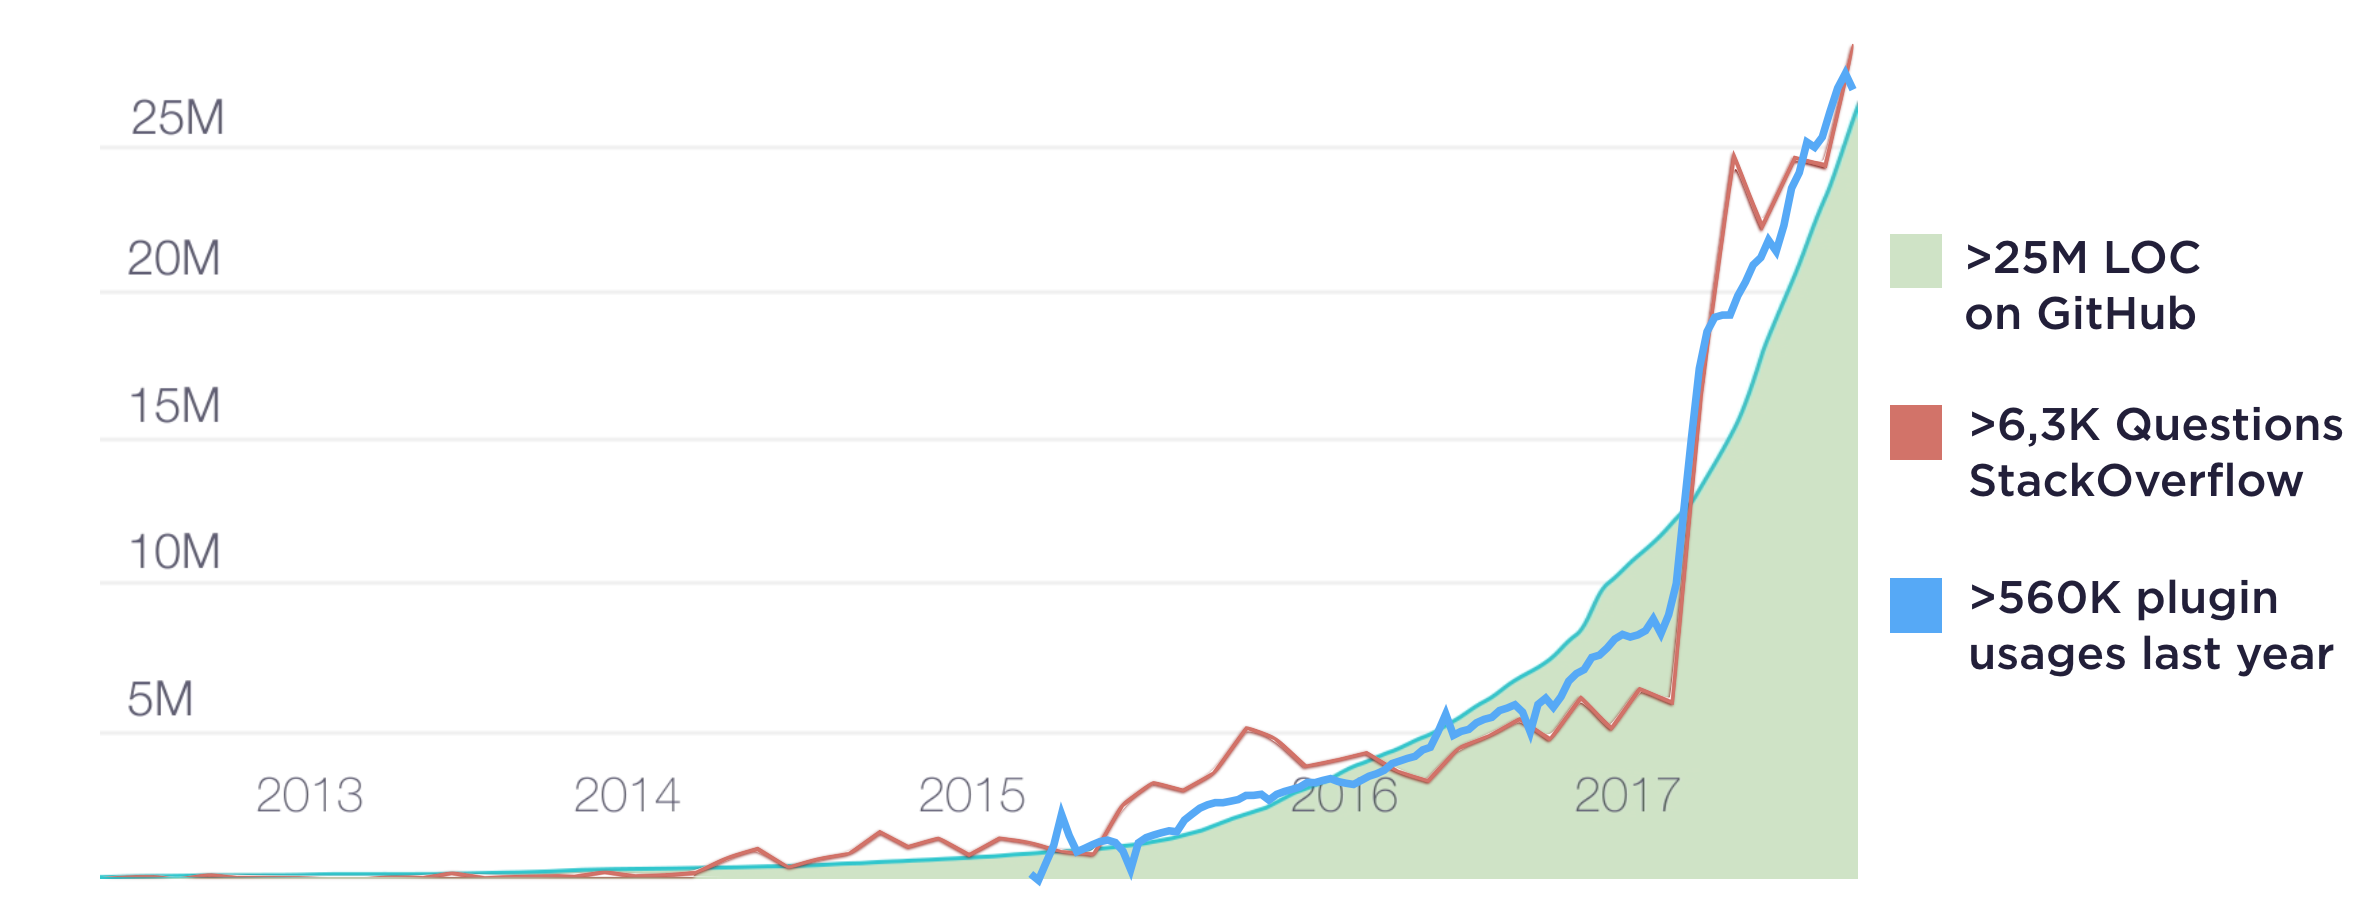
\includegraphics[width=0.95\textwidth]{img/KotlinAdoption.png}
	\caption{Hoeveelheid Github code in Kotlin \cite{JetBrains12}}
	\label{fig:kotlingithub}
\end{figure}

\begin{figure} [ht]
	\centering
	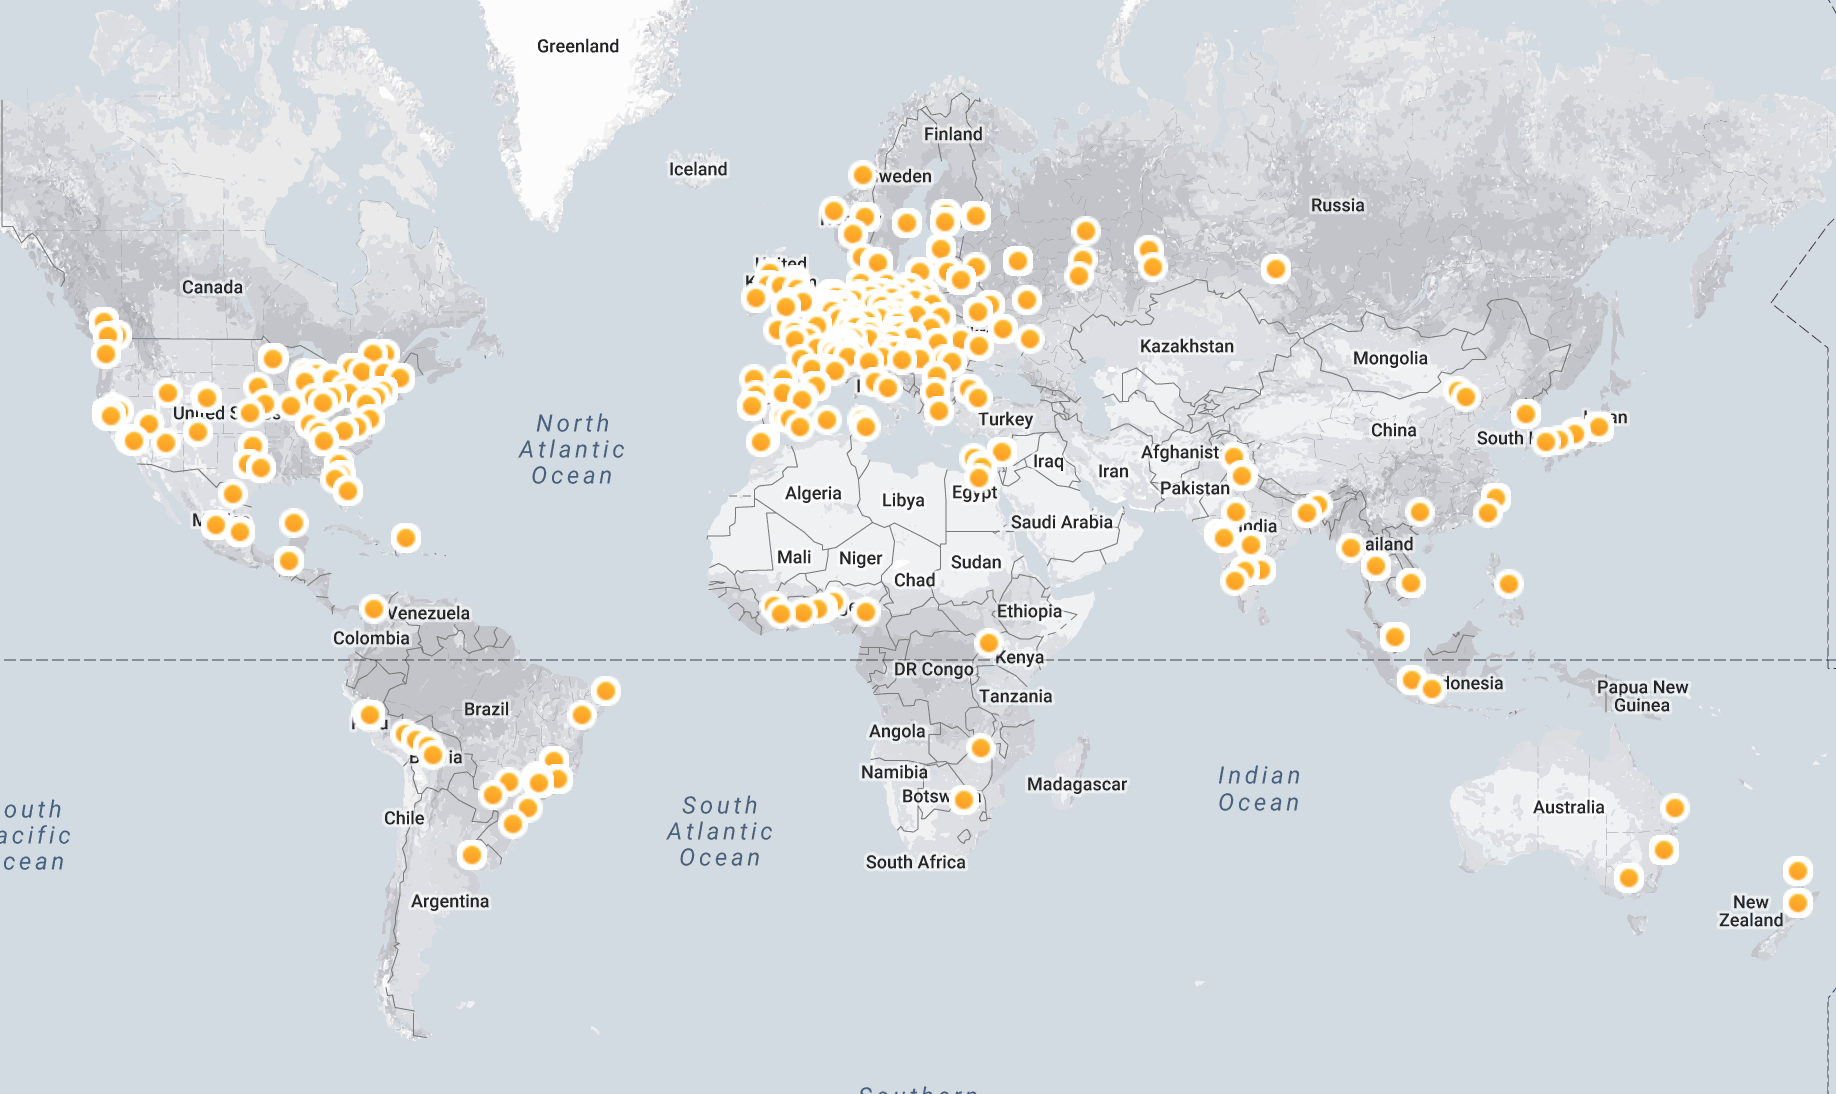
\includegraphics[width=0.95\textwidth]{img/KUGmap.png}
	\caption{User groups in de wereld \cite{JetBrains12}}
	\label{fig:usergroups}
\end{figure}

Volgens statistieken van een Android software ontwikkelingsbedrijf genaamd \textcite{AppBrain}, is Kotlin het beste framework voor Android applicaties te ontwikkelen. Verschillende belangrijke en veel gebruikte applicaties zoals Netflix, Twitter, Candy Crash bevatten grote delen Kotlin code.

Deze tweede figuur toont de verschillende user groups over de volledige wereld. Het toont aan dat Kotlin toch zeer veel gebruikt worden in onze streken.

\section{Waarom Kotlin?}
\label{sec:whykotlin}
Maar waarom heeft JetBrains nu besloten te beginnen met een nieuwe programmeertaal en deze dan later verder uit te bouwen met een cross-platform framework?

Een verklaring die men vaak leest op het internet, is dat JetBrains Kotlin uitvond omdat ze niet tevreden waren met Java en hun eigen productiviteit wilden vergroten. Ze vonden dus Java in sommige aspecten 'slecht'. JetBrains is een ontwikkelaar van IDE's die geschreven worden in Java, en dit is waar het schoentje wringt. Aangezien ze zelf vinden dat Java gebreken heeft, moesten ze met een oplossing komen: Kotlin.

Anderzijds het feit dat ze kiezen voor een taal die draait op de JVM, betekent dus dat men niet alle bestaande libraries willen herschrijven, maar hergebruiken.

%Dit hoofdstuk bevat je literatuurstudie. De inhoud gaat verder op de inleiding, maar zal het onderwerp van de bachelorproef *diepgaand* uitspitten. De bedoeling is dat de lezer na lezing van dit hoofdstuk helemaal op de hoogte is van de huidige stand van zaken (state-of-the-art) in het onderzoeksdomein. Iemand die niet vertrouwd is met het onderwerp, weet er nu voldoende om de rest van het verhaal te kunnen volgen, zonder dat die er nog andere informatie moet over opzoeken \autocite{Pollefliet2011}.

%Je verwijst bij elke bewering die je doet, vakterm die je introduceert, enz. naar je bronnen. In \LaTeX{} kan dat met het commando \texttt{$\backslash${textcite\{\}}} of \texttt{$\backslash${autocite\{\}}}. Als argument van het commando geef je de ``sleutel'' van een ``record'' in een bibliografische databank in het Bib\TeX{}-formaat (een tekstbestand). Als je expliciet naar de auteur verwijst in de zin, gebruik je \texttt{$\backslash${}textcite\{\}}.
%Soms wil je de auteur niet expliciet vernoemen, dan gebruik je \texttt{$\backslash${}autocite\{\}}. In de volgende paragraaf een voorbeeld van elk.

%\textcite{Knuth1998} schreef een van de standaardwerken over sorteer- en zoekalgoritmen. Experten zijn het erover eens dat cloud computing een interessante opportuniteit vormen, zowel voor gebruikers als voor dienstverleners op vlak van informatietechnologie~\autocite{Creeger2009}.

%\lipsum[7-20]
